\subsection{Entanglement}
Chains become entangled, because every block is shared between peers.
Every block is present in two chains and references the previous block of node A and of node B.
The chains quickly form a large graph with every node in the graph representing a block.
Every node has two outward directed edges and two incoming directed edges
except the nodes representing the genesis block and the most recent block.
The outward edges point to the previous blocks
and the incoming edges come from the next block in chronological ordering.

An simple example of three blocks can be seen in Figure \ref{fig:chain-example}.
In this example the first block contains a transaction between peer A and B.
This block references the previous block of both A and B.
Peer A continues with a transaction with C and peer B transacts with D.
Now the previous hash of A and B is the same as they share a block on their chains.
This hash is used in different transactions.
Color has been added to denote the direction of the chain of peers.

\begin{figure}[ht]
	\centerline{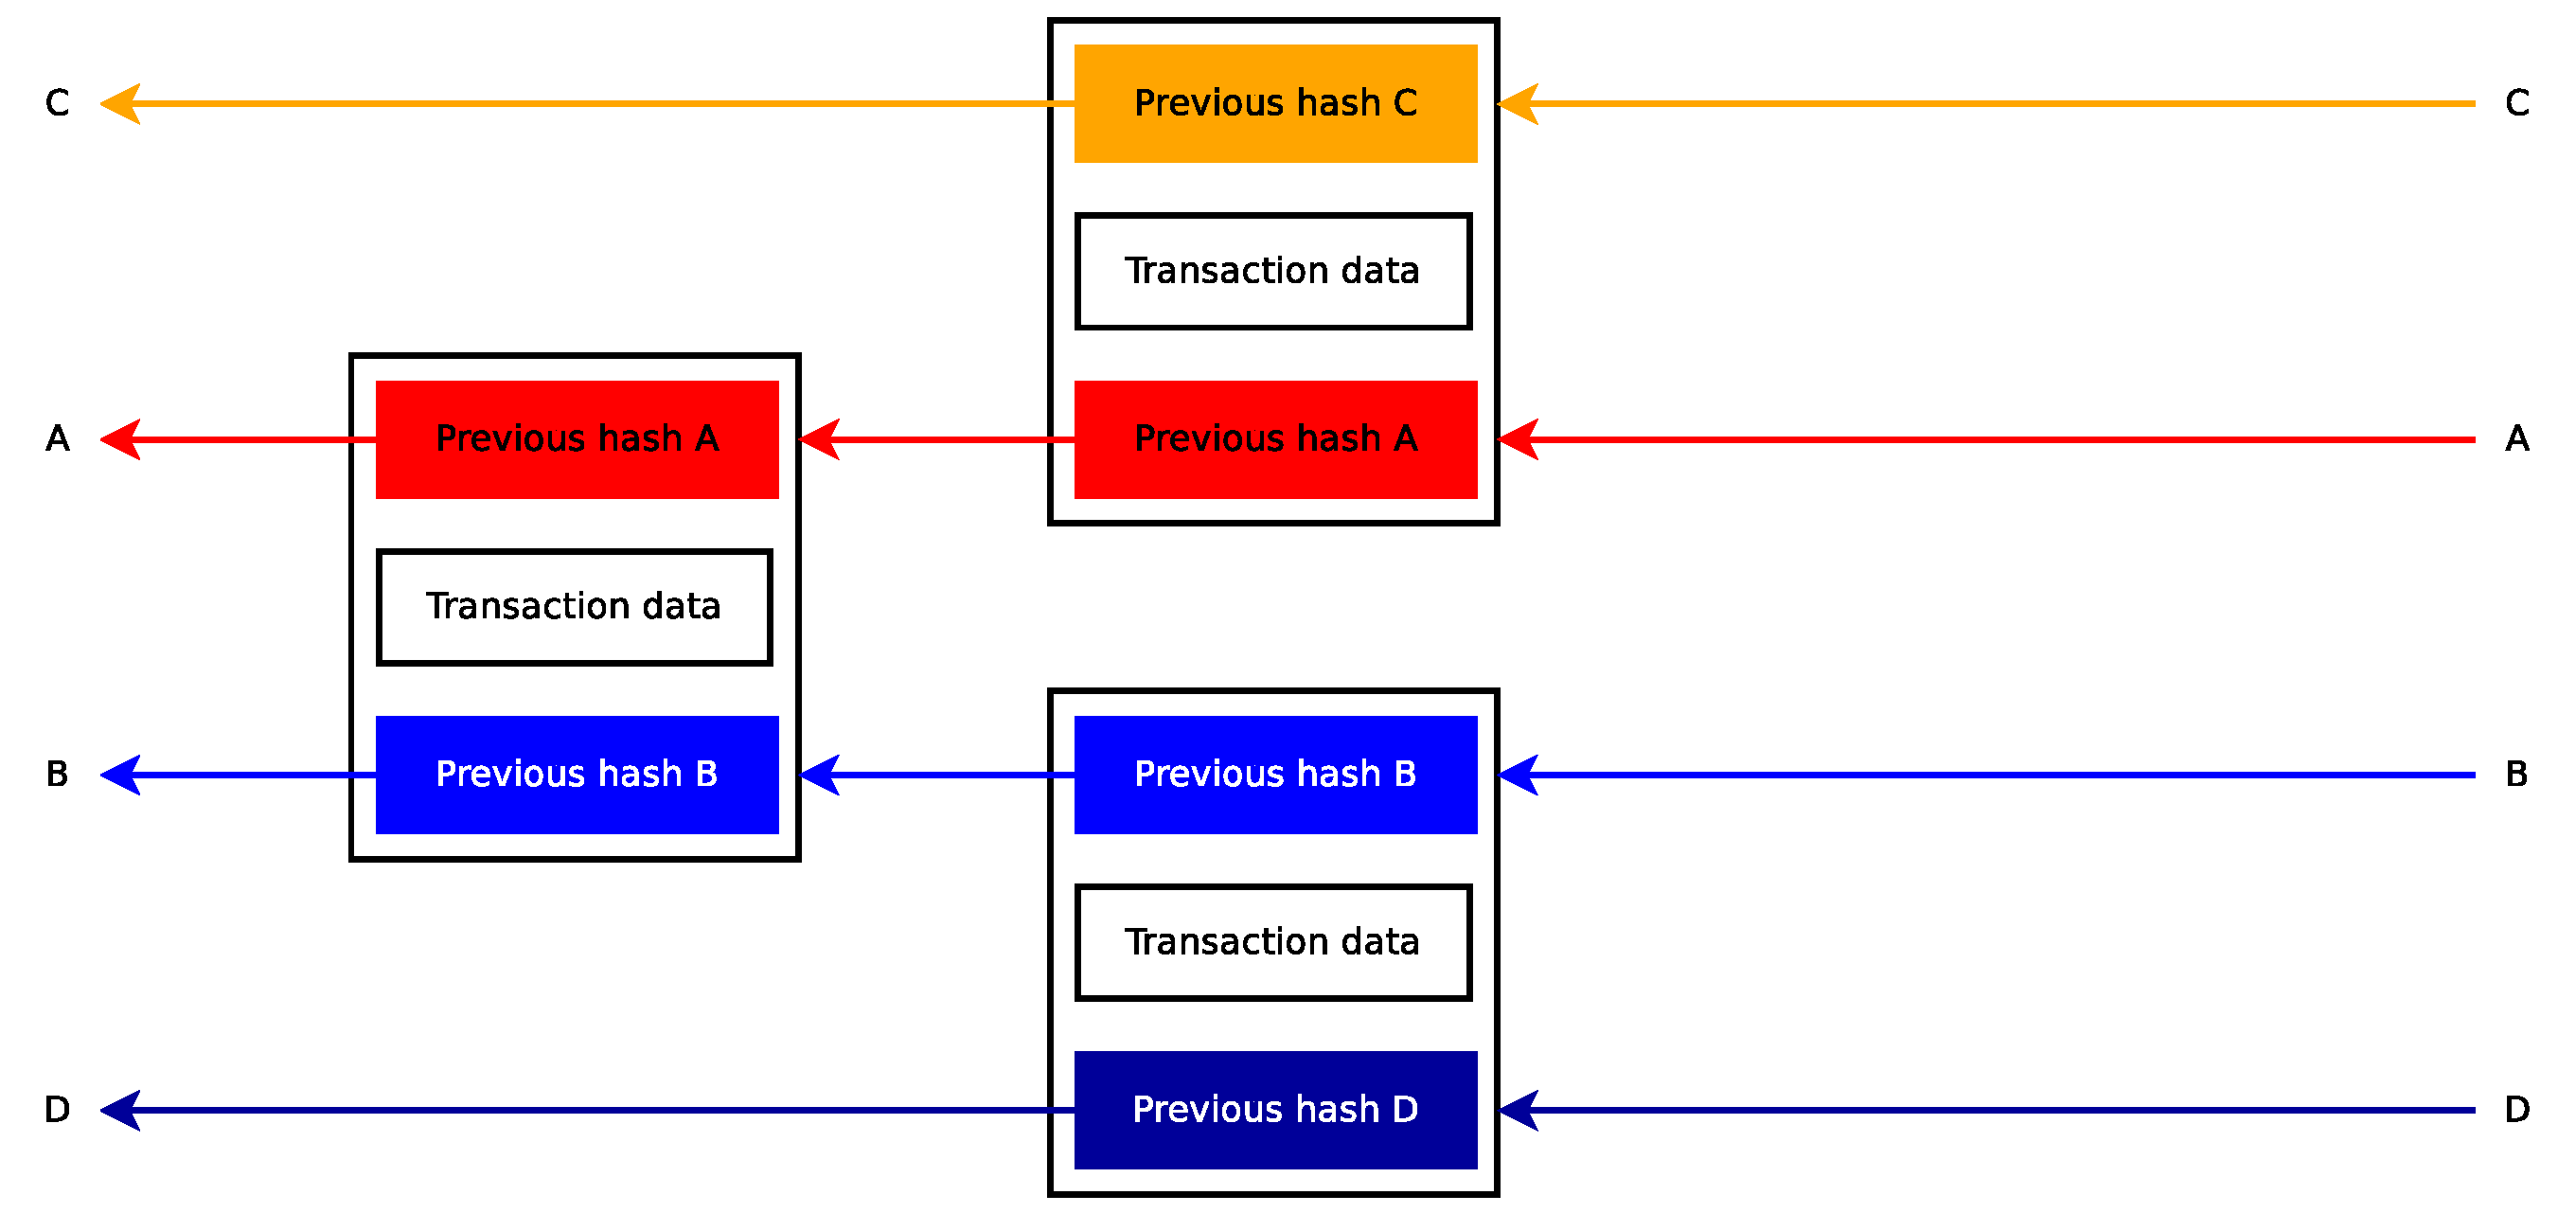
\includegraphics[scale=0.3]{design/figs/entangled-chain.eps}}
	\caption{Entanglement of chains within MultiChain.}
	\label{fig:chain-example}
\end{figure}


